\documentclass{article}
\usepackage{graphicx}
\usepackage{amsmath}
% Note: composable package will be auto-injected by cstex

\title{CSF Paper Template with Automatic Linking}
\author{Your Name}
\date{\today}

\begin{document}

\maketitle

\section{Introduction}

This is a sample paper created with the Composable Science Framework.
All computational steps are reproducible and verifiable through automatically
embedded provenance links.

\section{Results}

\begin{figure}[h]
\centering
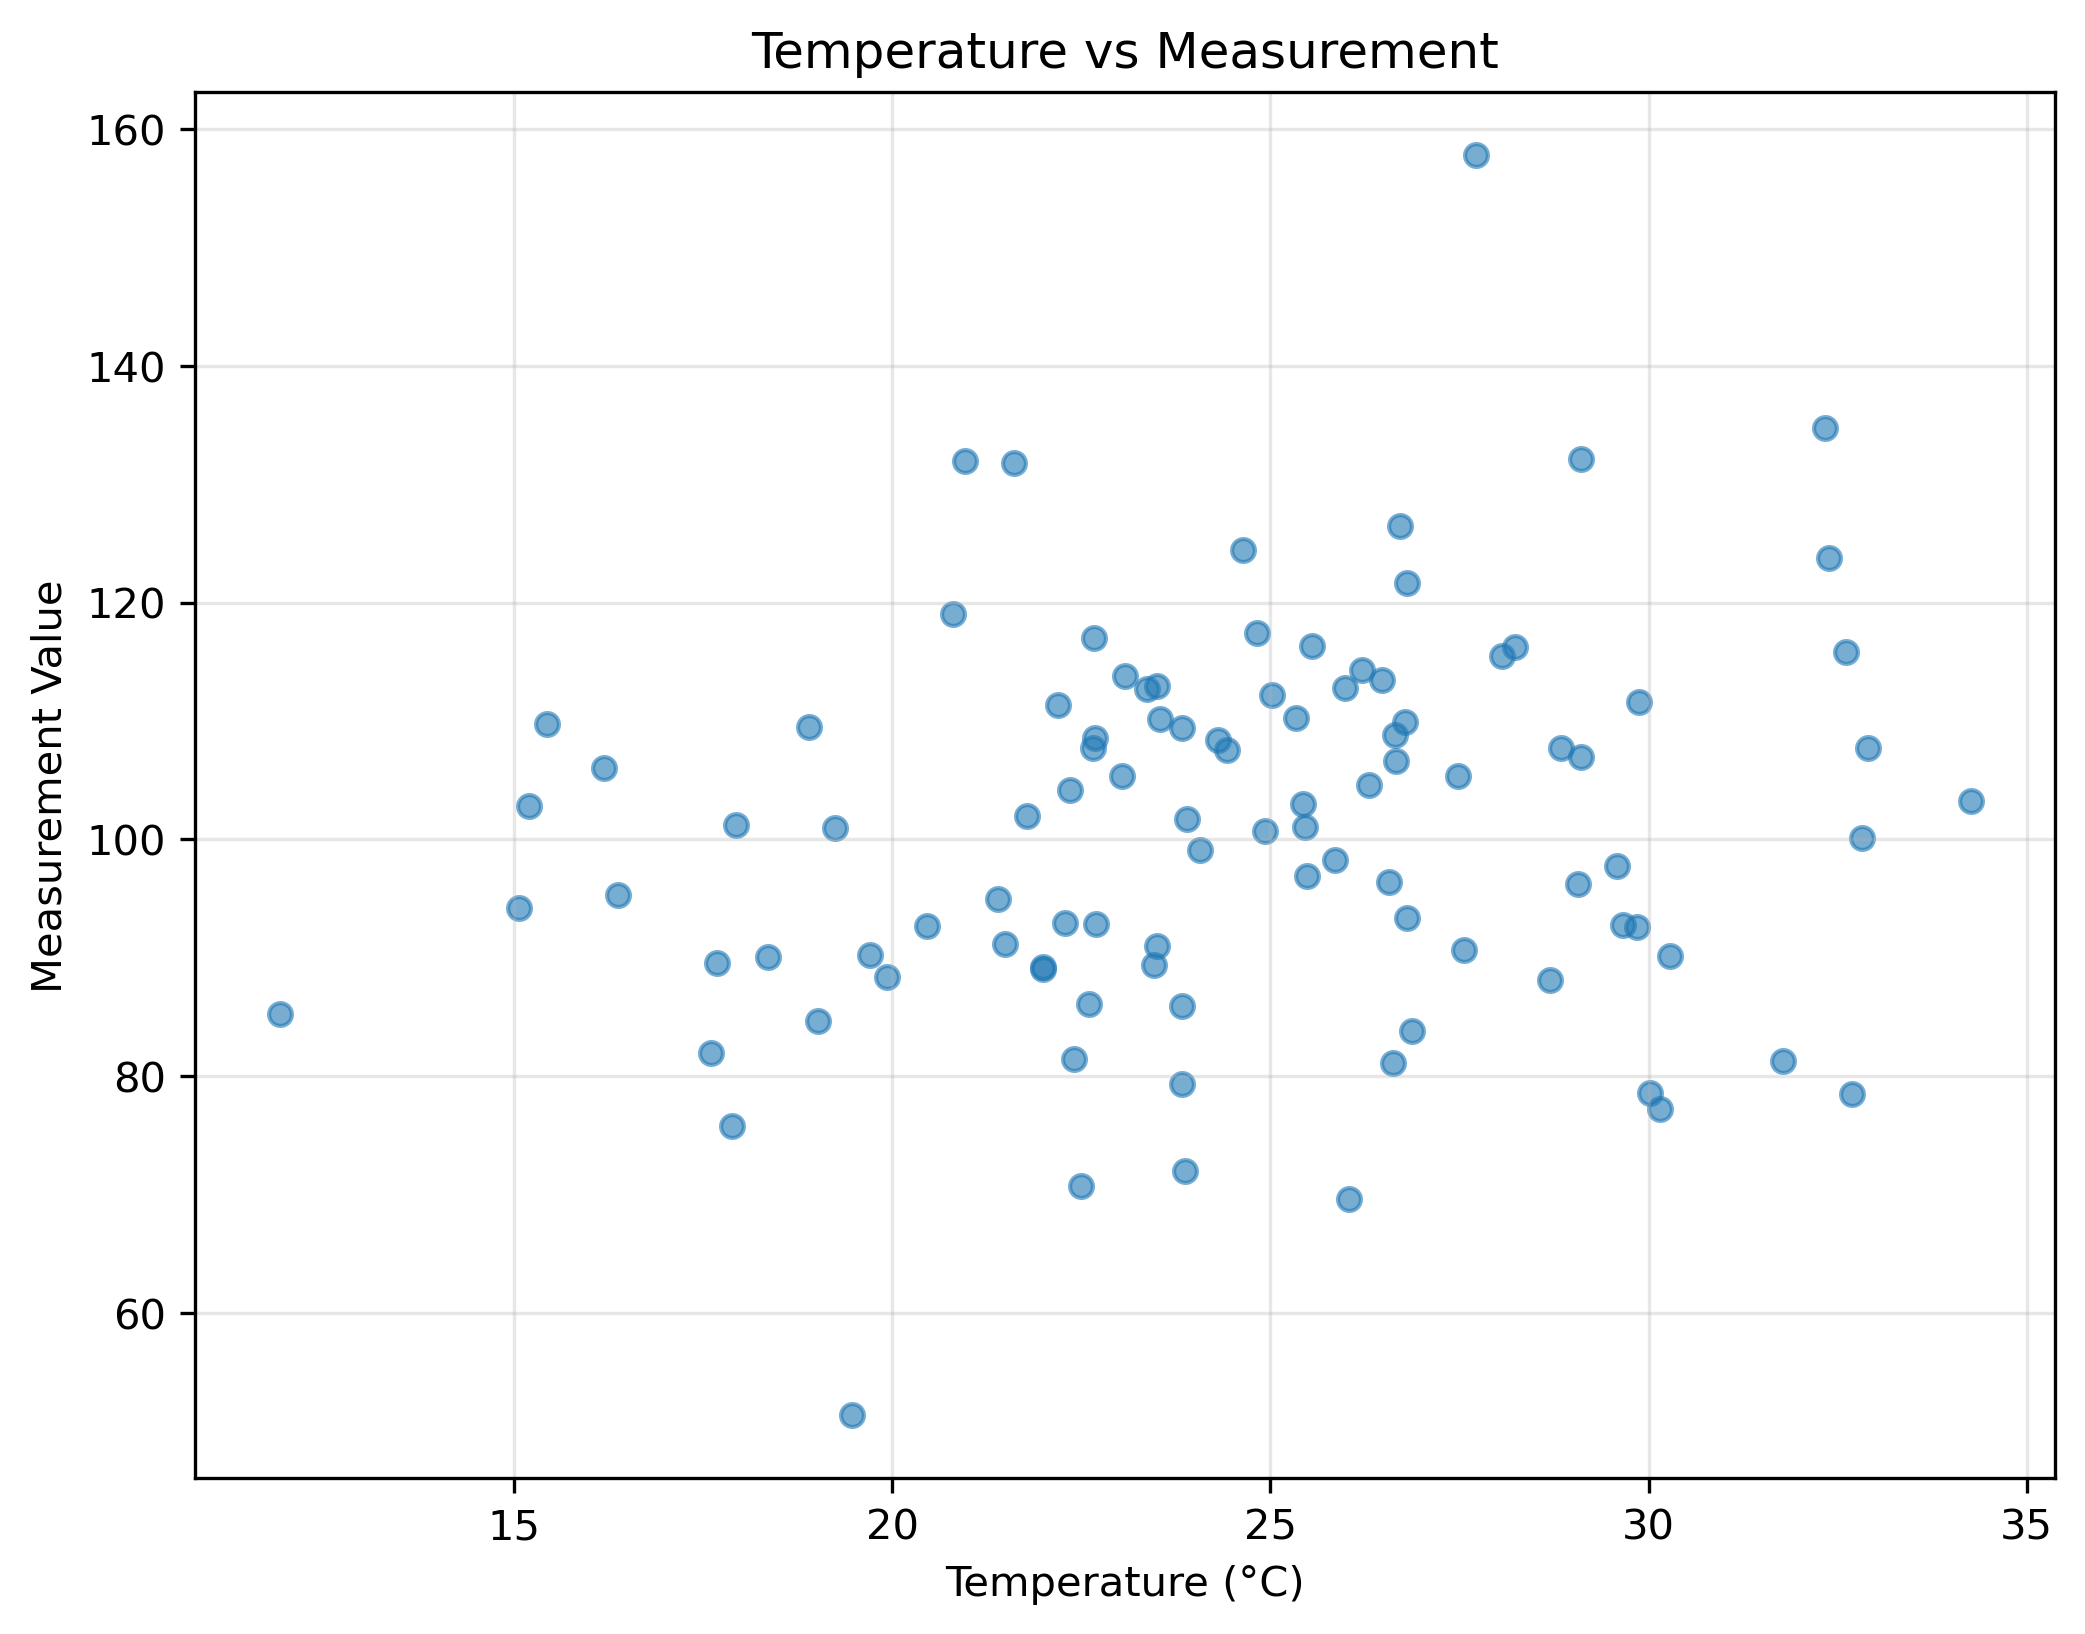
\includegraphics[width=0.8\textwidth]{figures/temperature_measurement.png}
\caption{Temperature vs Measurement Analysis showing the relationship between temperature and measurement values from our reproducible computation}
\label{fig:temperature}
\end{figure}

Figure \ref{fig:temperature} demonstrates the correlation between temperature
and measurements. The computational provenance link is automatically embedded
by the \texttt{cstex} compiler, allowing readers to verify the exact code and
data that generated this visualization.

\begin{figure}[h]
\centering
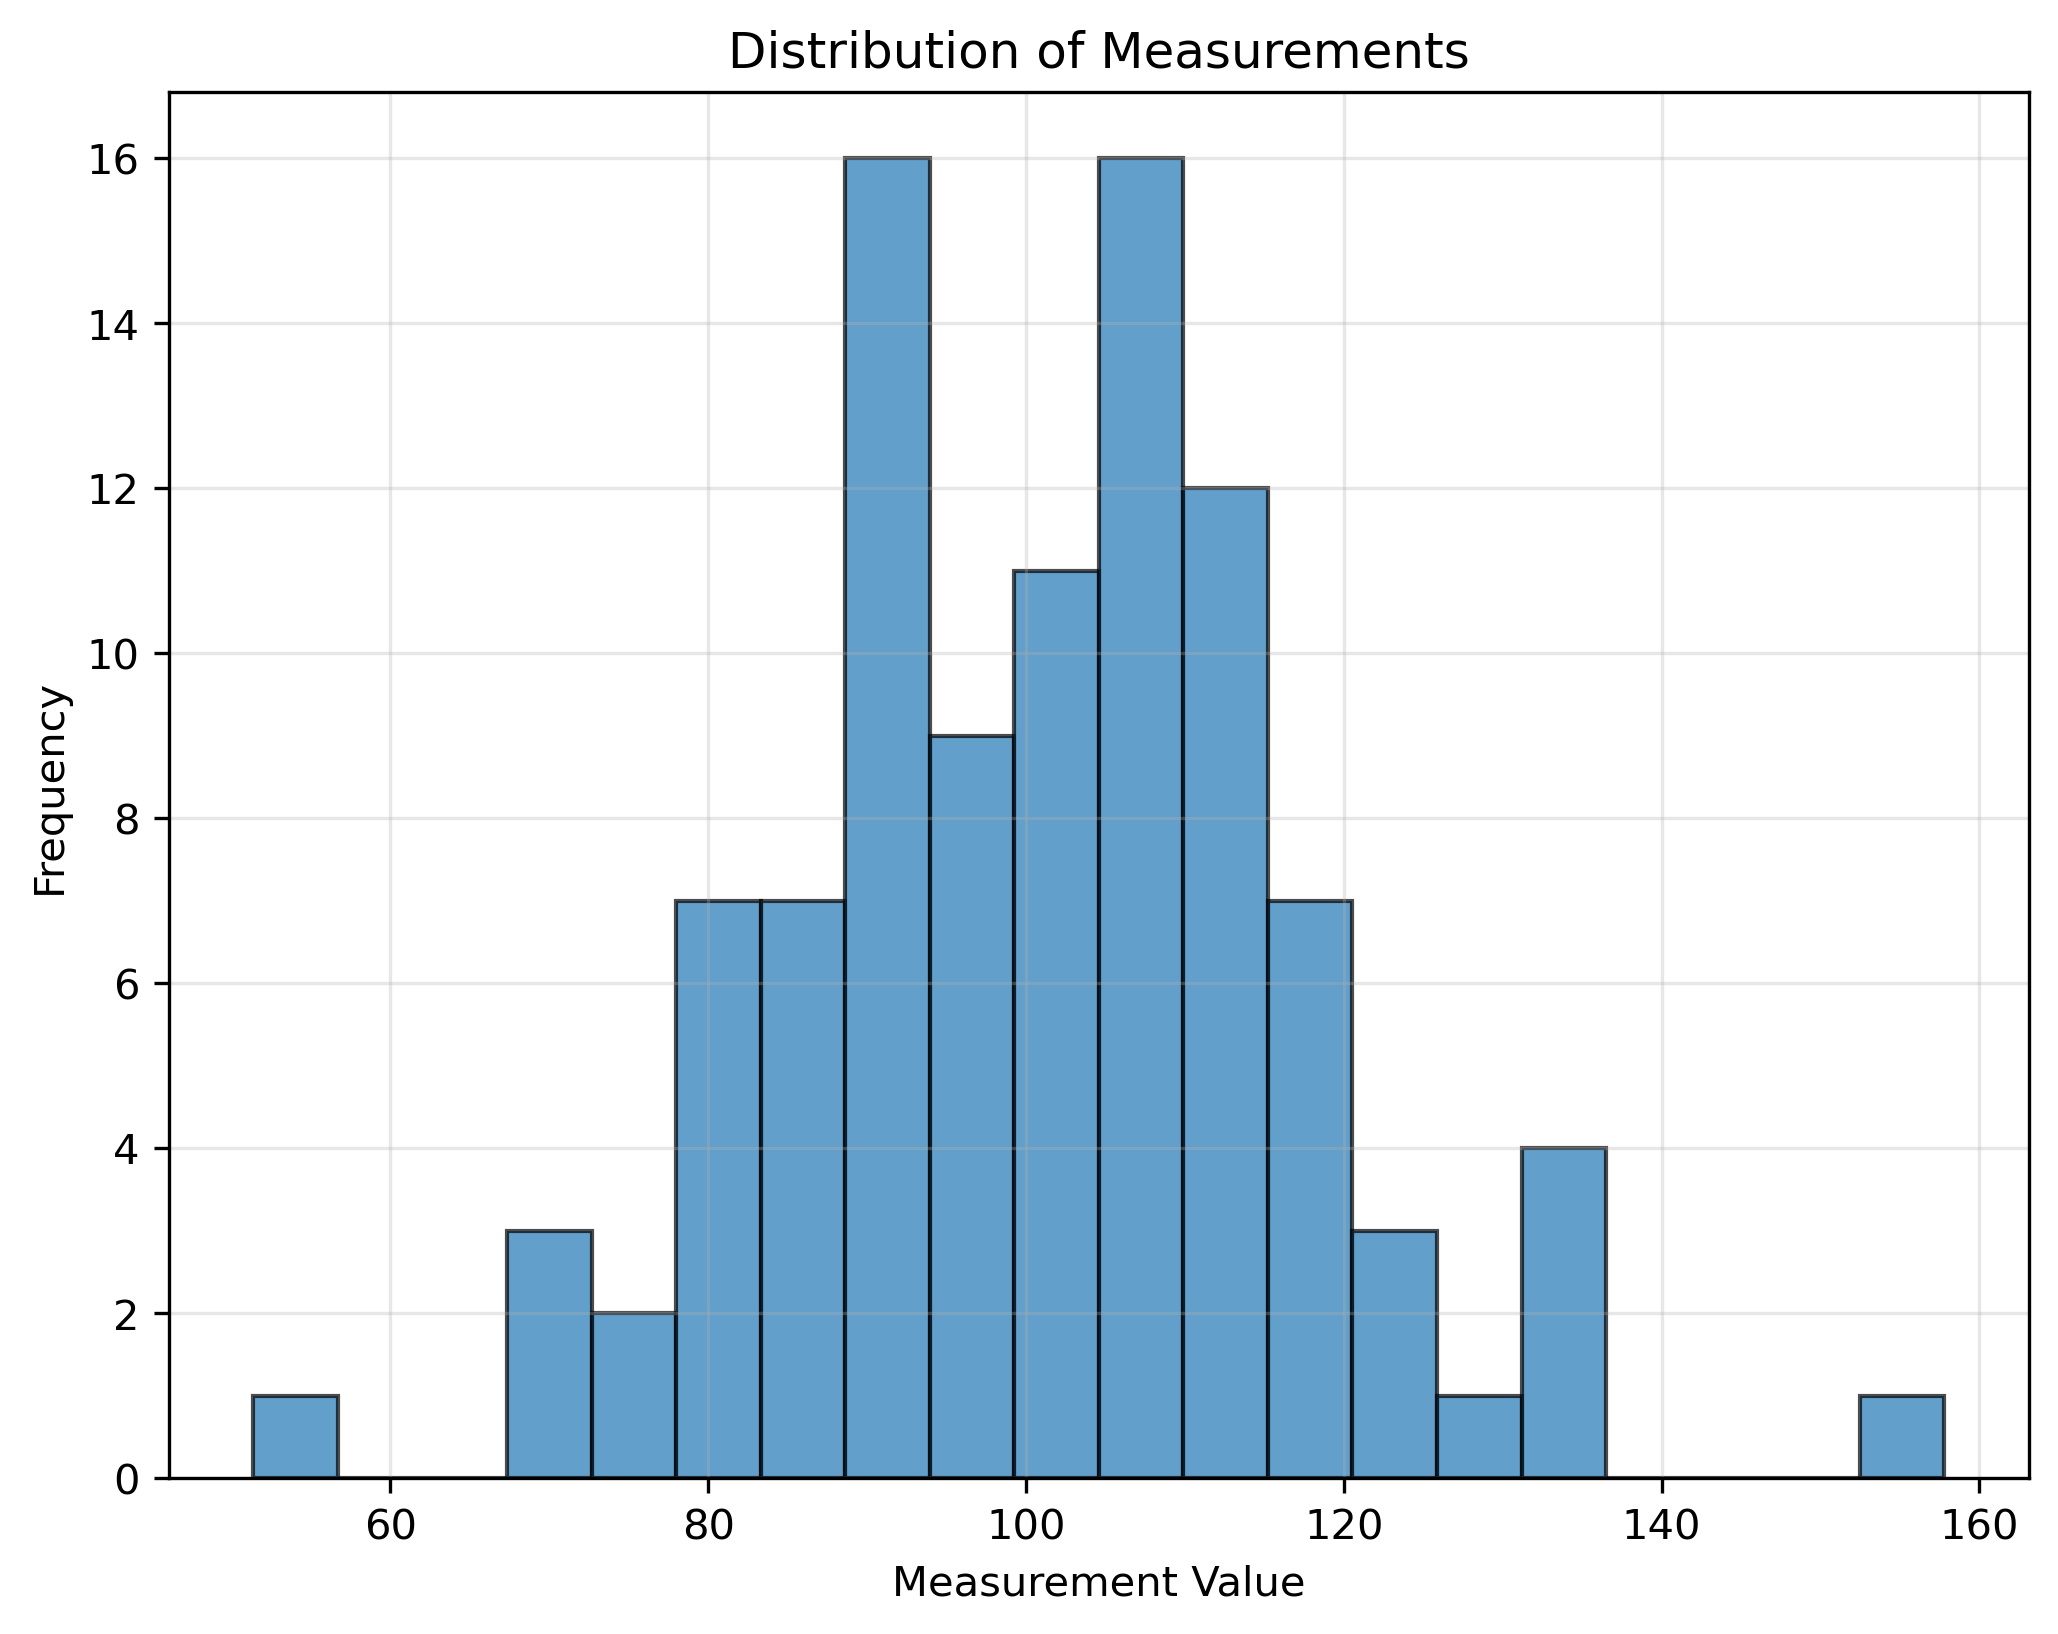
\includegraphics[width=0.7\textwidth]{figures/measurement_distribution.png}
\caption{Distribution of measurements showing the statistical properties of our dataset}
\label{fig:distribution}
\end{figure}

The histogram in Figure \ref{fig:distribution} provides insight into the
distribution characteristics of our measurements. No manual metadata
specification is required - \texttt{cstex} automatically discovers that this
figure is generated by the \texttt{figures} pipeline step.

\section{Methodology}

All figures in this paper are generated through the CSF pipeline defined
in \texttt{composable.toml}. The three-step process includes:

\begin{enumerate}
    \item \textbf{Data generation} (\texttt{scripts/generate\_sample\_data.py})
    \item \textbf{Figure creation} (\texttt{scripts/make\_figures.py})
    \item \textbf{Document compilation} (this LaTeX document)
\end{enumerate}

Each step is cryptographically attested and automatically linked to its
computational context by the \texttt{cstex} compilation process.

\section{Building This Document}

This document is compiled using the CSF-enhanced LaTeX toolchain:

\begin{verbatim}
# Automatic compilation with CSF integration
nix run github:composable-science/cstex#compile -- paper.tex

# Live preview with real-time provenance updates  
nix run github:composable-science/cstex#preview -- paper.tex
\end{verbatim}

The \texttt{cstex} compiler automatically:
\begin{itemize}
    \item Analyzes the pipeline to understand artifact provenance
    \item Discovers computational artifacts referenced in the document
    \item Injects provenance links without changing the source LaTeX
    \item Generates dashboard URLs for verification and reproduction
\end{itemize}

\section{Conclusion}

This paper demonstrates the new CSF paradigm where computational transparency
is achieved through intelligent tooling rather than manual annotation.
The \texttt{cstex} wrapper around \texttt{texMini} provides seamless
integration between documents and their computational provenance, enabling
unprecedented transparency in scientific communication with zero additional
effort from authors.

\end{document}
